% Options for packages loaded elsewhere
\PassOptionsToPackage{unicode}{hyperref}
\PassOptionsToPackage{hyphens}{url}
%
\documentclass[
  12pt,
]{article}
\title{Pre-workshop material - Workshop SVEPM 2022}
\usepackage{etoolbox}
\makeatletter
\providecommand{\subtitle}[1]{% add subtitle to \maketitle
  \apptocmd{\@title}{\par {\large #1 \par}}{}{}
}
\makeatother
\subtitle{Substantiating freedom from infection - available statistical
methods to prove freedom from infection in an output-based framework}
\author{Eleftherios Meletis, Aurélien Madouasse}
\date{2022-02-24}

\usepackage{amsmath,amssymb}
\usepackage{lmodern}
\usepackage{iftex}
\ifPDFTeX
  \usepackage[T1]{fontenc}
  \usepackage[utf8]{inputenc}
  \usepackage{textcomp} % provide euro and other symbols
\else % if luatex or xetex
  \usepackage{unicode-math}
  \defaultfontfeatures{Scale=MatchLowercase}
  \defaultfontfeatures[\rmfamily]{Ligatures=TeX,Scale=1}
\fi
% Use upquote if available, for straight quotes in verbatim environments
\IfFileExists{upquote.sty}{\usepackage{upquote}}{}
\IfFileExists{microtype.sty}{% use microtype if available
  \usepackage[]{microtype}
  \UseMicrotypeSet[protrusion]{basicmath} % disable protrusion for tt fonts
}{}
\makeatletter
\@ifundefined{KOMAClassName}{% if non-KOMA class
  \IfFileExists{parskip.sty}{%
    \usepackage{parskip}
  }{% else
    \setlength{\parindent}{0pt}
    \setlength{\parskip}{6pt plus 2pt minus 1pt}}
}{% if KOMA class
  \KOMAoptions{parskip=half}}
\makeatother
\usepackage{xcolor}
\IfFileExists{xurl.sty}{\usepackage{xurl}}{} % add URL line breaks if available
\IfFileExists{bookmark.sty}{\usepackage{bookmark}}{\usepackage{hyperref}}
\hypersetup{
  pdftitle={Pre-workshop material - Workshop SVEPM 2022},
  pdfauthor={Eleftherios Meletis, Aurélien Madouasse},
  hidelinks,
  pdfcreator={LaTeX via pandoc}}
\urlstyle{same} % disable monospaced font for URLs
\usepackage[margin=1in]{geometry}
\usepackage{color}
\usepackage{fancyvrb}
\newcommand{\VerbBar}{|}
\newcommand{\VERB}{\Verb[commandchars=\\\{\}]}
\DefineVerbatimEnvironment{Highlighting}{Verbatim}{commandchars=\\\{\}}
% Add ',fontsize=\small' for more characters per line
\usepackage{framed}
\definecolor{shadecolor}{RGB}{248,248,248}
\newenvironment{Shaded}{\begin{snugshade}}{\end{snugshade}}
\newcommand{\AlertTok}[1]{\textcolor[rgb]{0.94,0.16,0.16}{#1}}
\newcommand{\AnnotationTok}[1]{\textcolor[rgb]{0.56,0.35,0.01}{\textbf{\textit{#1}}}}
\newcommand{\AttributeTok}[1]{\textcolor[rgb]{0.77,0.63,0.00}{#1}}
\newcommand{\BaseNTok}[1]{\textcolor[rgb]{0.00,0.00,0.81}{#1}}
\newcommand{\BuiltInTok}[1]{#1}
\newcommand{\CharTok}[1]{\textcolor[rgb]{0.31,0.60,0.02}{#1}}
\newcommand{\CommentTok}[1]{\textcolor[rgb]{0.56,0.35,0.01}{\textit{#1}}}
\newcommand{\CommentVarTok}[1]{\textcolor[rgb]{0.56,0.35,0.01}{\textbf{\textit{#1}}}}
\newcommand{\ConstantTok}[1]{\textcolor[rgb]{0.00,0.00,0.00}{#1}}
\newcommand{\ControlFlowTok}[1]{\textcolor[rgb]{0.13,0.29,0.53}{\textbf{#1}}}
\newcommand{\DataTypeTok}[1]{\textcolor[rgb]{0.13,0.29,0.53}{#1}}
\newcommand{\DecValTok}[1]{\textcolor[rgb]{0.00,0.00,0.81}{#1}}
\newcommand{\DocumentationTok}[1]{\textcolor[rgb]{0.56,0.35,0.01}{\textbf{\textit{#1}}}}
\newcommand{\ErrorTok}[1]{\textcolor[rgb]{0.64,0.00,0.00}{\textbf{#1}}}
\newcommand{\ExtensionTok}[1]{#1}
\newcommand{\FloatTok}[1]{\textcolor[rgb]{0.00,0.00,0.81}{#1}}
\newcommand{\FunctionTok}[1]{\textcolor[rgb]{0.00,0.00,0.00}{#1}}
\newcommand{\ImportTok}[1]{#1}
\newcommand{\InformationTok}[1]{\textcolor[rgb]{0.56,0.35,0.01}{\textbf{\textit{#1}}}}
\newcommand{\KeywordTok}[1]{\textcolor[rgb]{0.13,0.29,0.53}{\textbf{#1}}}
\newcommand{\NormalTok}[1]{#1}
\newcommand{\OperatorTok}[1]{\textcolor[rgb]{0.81,0.36,0.00}{\textbf{#1}}}
\newcommand{\OtherTok}[1]{\textcolor[rgb]{0.56,0.35,0.01}{#1}}
\newcommand{\PreprocessorTok}[1]{\textcolor[rgb]{0.56,0.35,0.01}{\textit{#1}}}
\newcommand{\RegionMarkerTok}[1]{#1}
\newcommand{\SpecialCharTok}[1]{\textcolor[rgb]{0.00,0.00,0.00}{#1}}
\newcommand{\SpecialStringTok}[1]{\textcolor[rgb]{0.31,0.60,0.02}{#1}}
\newcommand{\StringTok}[1]{\textcolor[rgb]{0.31,0.60,0.02}{#1}}
\newcommand{\VariableTok}[1]{\textcolor[rgb]{0.00,0.00,0.00}{#1}}
\newcommand{\VerbatimStringTok}[1]{\textcolor[rgb]{0.31,0.60,0.02}{#1}}
\newcommand{\WarningTok}[1]{\textcolor[rgb]{0.56,0.35,0.01}{\textbf{\textit{#1}}}}
\usepackage{graphicx}
\makeatletter
\def\maxwidth{\ifdim\Gin@nat@width>\linewidth\linewidth\else\Gin@nat@width\fi}
\def\maxheight{\ifdim\Gin@nat@height>\textheight\textheight\else\Gin@nat@height\fi}
\makeatother
% Scale images if necessary, so that they will not overflow the page
% margins by default, and it is still possible to overwrite the defaults
% using explicit options in \includegraphics[width, height, ...]{}
\setkeys{Gin}{width=\maxwidth,height=\maxheight,keepaspectratio}
% Set default figure placement to htbp
\makeatletter
\def\fps@figure{htbp}
\makeatother
\setlength{\emergencystretch}{3em} % prevent overfull lines
\providecommand{\tightlist}{%
  \setlength{\itemsep}{0pt}\setlength{\parskip}{0pt}}
\setcounter{secnumdepth}{-\maxdimen} % remove section numbering
\ifLuaTeX
  \usepackage{selnolig}  % disable illegal ligatures
\fi

\begin{document}
\maketitle

\hypertarget{overview}{%
\section{Overview}\label{overview}}

This document will help you to prepare for the workshop on the available
statistical methods to prove freedom from infection in an output-based
framework, that will be held in the SVEPM conference on 23 March 2022.
The workshop involves both demonstration and hands-on training, so it is
very important that you are using a computer with the necessary software
installed. All training material, presented during this workshop, will
be available for download from the GitHub site, so you might find it
helpful to create a GitHub account, before the workshop. The purpose of
this document is to ensure that you have the necessary software
installed, access to the GitHub repository, download all training
material, and to give you a brief introduction in the topic of this
workshop e.g., terminology etc.

Required time: 2 hours

\hypertarget{software-installation}{%
\section{Software installation}\label{software-installation}}

You need to install R (version 4.0.0 or later) from
\url{https://cran.r-project.org/} and we recommend that you also use
Rstudio which can be downloaded separately from
\url{https://www.rstudio.com/products/rstudio/download/}

Please also install the latest versions of the following R packages from
CRAN (or using the install.packages() function): tidyverse, PriorGen,
rjags, runjags, posterior, coda, TeachingDemos, ggmcmc, devtools,
remotes

Example: Install more than one package using install.packages()
function:

\begin{Shaded}
\begin{Highlighting}[]
\CommentTok{\#install.packages(c("tidyverse", "PriorGen"))}
\end{Highlighting}
\end{Shaded}

You will also need the standalone JAGS software (version 4.3.0 or later)
for the workshop - download the installer for your platform from here:
\url{https://sourceforge.net/projects/mcmc-jags/files/JAGS/4.x/}

To check that you have installed the software correctly please run the
following code within R (or RStudio) and make sure that no errors are
produced:

\begin{Shaded}
\begin{Highlighting}[]
\FunctionTok{stopifnot}\NormalTok{(}\FunctionTok{getRversion}\NormalTok{() }\SpecialCharTok{\textgreater{}=} \StringTok{"4.0.0"}\NormalTok{)}
\CommentTok{\#stopifnot(require(\textquotesingle{}tidyverse\textquotesingle{}))}
\FunctionTok{stopifnot}\NormalTok{(}\FunctionTok{require}\NormalTok{(}\StringTok{\textquotesingle{}PriorGen\textquotesingle{}}\NormalTok{))}
\FunctionTok{stopifnot}\NormalTok{(}\FunctionTok{require}\NormalTok{(}\StringTok{\textquotesingle{}rjags\textquotesingle{}}\NormalTok{))}
\FunctionTok{stopifnot}\NormalTok{(}\FunctionTok{require}\NormalTok{(}\StringTok{\textquotesingle{}runjags\textquotesingle{}}\NormalTok{))}
\FunctionTok{stopifnot}\NormalTok{(}\FunctionTok{require}\NormalTok{(}\StringTok{\textquotesingle{}coda\textquotesingle{}}\NormalTok{))}
\FunctionTok{stopifnot}\NormalTok{(}\FunctionTok{require}\NormalTok{(}\StringTok{\textquotesingle{}TeachingDemos\textquotesingle{}}\NormalTok{))}
\CommentTok{\#stopifnot(require(\textquotesingle{}ggmcmc\textquotesingle{}))}
\FunctionTok{stopifnot}\NormalTok{(}\FunctionTok{require}\NormalTok{(}\StringTok{\textquotesingle{}devtools\textquotesingle{}}\NormalTok{))}
\FunctionTok{stopifnot}\NormalTok{(}\FunctionTok{require}\NormalTok{(}\StringTok{"remotes"}\NormalTok{))}
\FunctionTok{stopifnot}\NormalTok{(}\FunctionTok{testjags}\NormalTok{()}\SpecialCharTok{$}\NormalTok{JAGS.available)}
\FunctionTok{stopifnot}\NormalTok{(}\FunctionTok{numeric\_version}\NormalTok{(}\FunctionTok{testjags}\NormalTok{()}\SpecialCharTok{$}\NormalTok{JAGS.version) }\SpecialCharTok{\textgreater{}=} \StringTok{"4.3.0"}\NormalTok{)}
\FunctionTok{stopifnot}\NormalTok{(}\FunctionTok{testjags}\NormalTok{()}\SpecialCharTok{$}\NormalTok{rjags.found)}
\FunctionTok{stopifnot}\NormalTok{(}\FunctionTok{numeric\_version}\NormalTok{(}\FunctionTok{testjags}\NormalTok{()}\SpecialCharTok{$}\NormalTok{rjags.version) }\SpecialCharTok{\textgreater{}=} \StringTok{"4{-}8"}\NormalTok{)}
\end{Highlighting}
\end{Shaded}

CmdStanR, stopifnot(require(`CmdStanR')) stopifnot(require(`posterior'))

Lastly, you need to install the STOCfree package and it's associated
R-packages (cmdstanr, posterior) from GitHub running the following code
within R (or RStudio):

\begin{Shaded}
\begin{Highlighting}[]
\NormalTok{remotes}\SpecialCharTok{::}\FunctionTok{install\_github}\NormalTok{(}\StringTok{"stan{-}dev/cmdstanr"}\NormalTok{)}
\end{Highlighting}
\end{Shaded}

\begin{verbatim}
## Skipping install of 'cmdstanr' from a github remote, the SHA1 (17c5e884) has not changed since last install.
##   Use `force = TRUE` to force installation
\end{verbatim}

\begin{Shaded}
\begin{Highlighting}[]
\CommentTok{\#install.packages("posterior")}
\end{Highlighting}
\end{Shaded}

Now you are ready to install from GitHub the STOCfree package runnig the
following code within R (or RStudio) and select option 1 to install all
update packages:

\begin{Shaded}
\begin{Highlighting}[]
\FunctionTok{library}\NormalTok{(devtools)}
\FunctionTok{install\_github}\NormalTok{(}\StringTok{"AurMad/STOCfree"}\NormalTok{)}
\end{Highlighting}
\end{Shaded}

\begin{verbatim}
## Skipping install of 'STOCfree' from a github remote, the SHA1 (6dd336b0) has not changed since last install.
##   Use `force = TRUE` to force installation
\end{verbatim}

Let's check is the STOCfree has been installed correctly

\begin{Shaded}
\begin{Highlighting}[]
\FunctionTok{stopifnot}\NormalTok{(}\FunctionTok{require}\NormalTok{(}\StringTok{"STOCfree"}\NormalTok{))}
\end{Highlighting}
\end{Shaded}

If you have any difficulties installing the software or get errors from
the code above, please let us know immediately so that we can resolve
these during the workshop.

\hypertarget{github}{%
\section{GitHub}\label{github}}

\hypertarget{basics}{%
\subsection{Basics}\label{basics}}

GitHub is an online code repository that in it's most basic form stores
the version history of any code project you are working on, and allows
you to go back in time to a previous version before someone introduced a
bug. It is particularly useful when collaborating with others because it
allows you to see who made a change, when it was made, and what the code
looked like before that. It also allows changes from different people to
be merged into the same central repository to ensure that nobody gets
out of sync with everybody else's code.

We will primarily be using GitHub as a way to disseminate the lecture
notes and R/JAGS code for the exercises on course, so you only need to
use the most basic features of GitHub (but it is a good thing to learn).

\hypertarget{simple-web-usage}{%
\subsection{Simple Web Usage}\label{simple-web-usage}}

We have created a public repository containing the teaching material for
the training school. This means that anyone can view the teaching
material at any time via the following website:
\url{https://github.com/LefMel/harmony_larissa_training}

You should see a number of folders listed with names
``Pre\_Course\_Material'', ``Day1'', ``Day2'' and ``Day3''. Within these
folders are files like like ``Session\_Preparation.Rmd'',
``Session\_Preparation.pdf'' etc. Each of the sessions for the training
school (including this preparation document) has a series of files: the
.Rmd is the original Rmarkdown document, and the .pdf and .html files
are created from these. You can click on any of these files to view
them, although of the different file formats the .pdf version is
probably easiest to download directly from the website. There are two
problems with this:

1 - You will likely encounter problems when copy/pasting R code from the
PDF files.

2 - If/when any of the files are updated, you will not get an automatic
update of the new version.

We therefore recommend that you follow the instructions below to clone
the repository directly to your computer.

\hypertarget{creating-an-account}{%
\subsection{Creating an Account}\label{creating-an-account}}

If you have never used GitHub before, you should create an account via
\url{http://github.com} - it is free and easy. Remember to make a note
of the username and password that you just created!

\hypertarget{github-desktop}{%
\subsection{GitHub Desktop}\label{github-desktop}}

The easiest way to use GitHub is via GitHub desktop. Go to
\url{https://desktop.github.com} and download/install the software. Then
open it and sign in using your GitHub account (the username and password
that you just created). This should become the primary way in which you
interact with GitHub, rather than via your browser.

The first step is to clone the \texttt{SVEPM\_2022\_wk} repository on to
your computer. From inside GitHub Desktop, go to the File menu then
Clone Respository, then click on the URL tab. Then type/paste
\texttt{LefMel/SVEPM\_2022\_wk} into the box where it says
\texttt{Filter\ your\ reposotories} or \texttt{Repository\ URL} or
\texttt{GitHub\ username\ and\ repository} (depending on your version of
GitHub Desktop). A suggested local path folder will be created
automatically at the bottom but feel free to change this. Then click on
Clone and wait for the files to download.

Creating the clone copies all of the files currently on the GitHub
repository to your computer at the local path specified above (if you
can't remember what this was choose `Show in Windows/Finder' or similar,
depending on your OS, under the Respository menu). This is where all of
the course material will (eventually) be located. For example, look
inside the
\texttt{\textquotesingle{}Pre\_Course\_Material\textquotesingle{}}
folder and open up the
\texttt{\textquotesingle{}Session\_Preparation.html\textquotesingle{}}
file - that is a local copy of the same document you are currently
reading! But now you also have the PDF version - use this if you want to
print the document for some reason, but it is a good idea to stick to
using the HTML version if you want to copy/paste R code (you will
probably encounter problems with quotation marks if you copy/paste R
code from PDF files). The two versions should be identical.

\hypertarget{modifying-files}{%
\subsection{Modifying Files}\label{modifying-files}}

Once you have set up the local copy of the repository, you can then add,
delete and modify any of the files within your local copy of the
repository. Try doing this by deleting the
\texttt{\textquotesingle{}Session\_Preparation.html\textquotesingle{}}
file. Now go back to GitHub Desktop where you should see a line appear
on the left with a red minus symbol in a box to the right hand side -
this is telling you that a file has been deleted locally (if you had
modified the file rather than deleting it, the box would be orange and
contain a dot). However, you don't want to delete or modify any of the
files we are providing in case we update them later. If you do this by
mistake, just right-click the relevant line in GitHub desktop and choose
``Discard changes'' - the file should then be restored. Do this now for
the
\texttt{\textquotesingle{}Session\_Preparation.html\textquotesingle{}}
file and check that it has reappeared. If you do want to modify a file
for some reason, we suggest that you copy it and modify the copied
version. If you keep the copy inside the same folder then GitHub desktop
will show the new file (green plus in the box) but you can safely ignore
these, or move the copied file outside of the repository folder if you
want to keep things simple.

\hypertarget{fetching-updates}{%
\subsection{Fetching Updates}\label{fetching-updates}}

An important advantage of GitHub is that we can update a file online
(for example to fix a typo or add new material discussed during the
workshop), and that update will be immediately available to all of you.
But in order to receive the updated files you need to tell GitHub
desktop to look for updates. Open GitHub desktop, then click on `Fetch
origin' and then `Pull' to make sure that any recent changes are synced
to your computer. As long as you remember to pull changes regularly then
you will always have an up-to-date copy - so do this regularly.
Forgetting to do this is the only real potential downside of Git.

\hypertarget{more-information}{%
\subsection{More information}\label{more-information}}

That is pretty much all you need to know for the training school but
there are some good tutorials available, for example:
\url{https://happygitwithr.com}.

\hypertarget{topics-of-this-workshop}{%
\section{Topics of this Workshop}\label{topics-of-this-workshop}}

\hypertarget{introduction}{%
\subsection{Introduction}\label{introduction}}

The aim of this pre-workshop material is to introduce the basics of the
current statistical methods to prove freedom from infection in an
output-based framework, that you will work on during the workshop. The
text and code below is designed so that you can become familiar both
with the terminology and the methods (especially Bayesian methods) that
will be discussed during the workshop. You can run the code shown and
check that your results agree with those shown here. If you have not
encountered a function before then consult the help file for that
function with a question mark followed by the function name, for
example: \texttt{?seq} . Some prior familiarity with R will be assumed
for this exercise but if you need to brush up then there are lots of
tutorials online
e.g.~\url{https://www.datacamp.com/courses/free-introduction-to-r}

We will assume that you have all worked through this material in advance
of the workshop.

\hypertarget{output-based-framework}{%
\subsection{Output-based framework}\label{output-based-framework}}

\hypertarget{probability-distributions}{%
\subsection{Probability distributions}\label{probability-distributions}}

Likelihood theory is at the heart of most inferential statistics - it
describes the chances of an event happening under certain assumptions,
such as the probability distribution and the parameter value(s) that we
want to use with that distribution. Put simply, a likelihood is the
probability of observing our data given the distribution that we use to
describe the data generating process. For example, what is the
likelihood (i.e.~probability) of getting 5 heads from 10 tosses of a
fair coin? Probability theory can help us decide - we can assume:

\begin{itemize}
\tightlist
\item
  The probability distribution describing a number of independent coin
  tosses is called the Binomial distribution
\item
  In this case, we would use the parameters:

  \begin{itemize}
  \tightlist
  \item
    Number of coin tosses = 10
  \item
    Probability of a head = `fair' = 0.5
  \end{itemize}
\end{itemize}

Wikipedia tells us that we can calculate the probability of a Binomial
distribution as follows:

\begin{Shaded}
\begin{Highlighting}[]
\NormalTok{tosses }\OtherTok{\textless{}{-}} \DecValTok{10}
\NormalTok{probability }\OtherTok{\textless{}{-}} \FloatTok{0.5}
\NormalTok{heads }\OtherTok{\textless{}{-}} \DecValTok{5}
\NormalTok{likelihood\_1 }\OtherTok{\textless{}{-}} \FunctionTok{choose}\NormalTok{(tosses, heads) }\SpecialCharTok{*}\NormalTok{ probability}\SpecialCharTok{\^{}}\NormalTok{heads }\SpecialCharTok{*}
\NormalTok{                (}\DecValTok{1}\SpecialCharTok{{-}}\NormalTok{probability)}\SpecialCharTok{\^{}}\NormalTok{(tosses}\SpecialCharTok{{-}}\NormalTok{heads)}
\NormalTok{likelihood\_1}
\end{Highlighting}
\end{Shaded}

\begin{verbatim}
## [1] 0.2460938
\end{verbatim}

But R makes our life easier by implementing this using a function called
dbinom:

\begin{Shaded}
\begin{Highlighting}[]
\NormalTok{likelihood\_2 }\OtherTok{\textless{}{-}} \FunctionTok{dbinom}\NormalTok{(heads, tosses, probability)}
\NormalTok{likelihood\_2}
\end{Highlighting}
\end{Shaded}

\begin{verbatim}
## [1] 0.2460938
\end{verbatim}

These two numbers are the same, which is reassuring. R also has a LOT of
other distributions, but the most common are:

\begin{itemize}
\tightlist
\item
  Discrete probability distributions

  \begin{itemize}
  \tightlist
  \item
    Binomial: dbinom
  \item
    Poisson: dpois
  \item
    Negative binomial: dnbinom
  \end{itemize}
\item
  Continuous probability distributions

  \begin{itemize}
  \tightlist
  \item
    Normal: dnorm
  \item
    Exponential: dexp
  \item
    Gamma: dgamma
  \item
    Beta: dbeta
  \item
    Lognormal: dlnorm
  \item
    Uniform: dunif
  \end{itemize}
\end{itemize}

If you are not familiar with these distributions, then you can take a
look them (and their common uses) on the internet.

\hypertarget{exercise-1---substantiating-freedom-from-infection-as-a-statistical-problem}{%
\subsection{Exercise 1 - Substantiating freedom from infection as a
statistical
problem}\label{exercise-1---substantiating-freedom-from-infection-as-a-statistical-problem}}

Imagine a large population in which 20\% of individuals are infected.
Although a random sample of 10 should contain 2 infected individuals on
average, each particular sample could include between 0 and 10 infected
individuals. Use the \texttt{dbinom} function to calculate the
probability of detecting 0 infected individuals. What does the output
represent? Change the values for the prevalence and the sample size and
see how the output varies.

\hypertarget{exercise-1---solution}{%
\subsection{Exercise 1 - Solution}\label{exercise-1---solution}}

\begin{Shaded}
\begin{Highlighting}[]
\CommentTok{\# x = 0, size = 10, prob = 0.2:}
\FunctionTok{dbinom}\NormalTok{(}\DecValTok{0}\NormalTok{,}\DecValTok{10}\NormalTok{,}\FloatTok{0.2}\NormalTok{)}
\end{Highlighting}
\end{Shaded}

The output probability representes the probability of freedom from
infection, meaning that there is 10.7\% that the population is
infection-free, assuming a sample of 10 individuals and a prevalence of
20\%.

Let's increase the prevalence at 40\%, i.e., prob = 0.4 and leave the
sample size same, i.e., size = 10.

\begin{Shaded}
\begin{Highlighting}[]
\FunctionTok{dbinom}\NormalTok{(}\DecValTok{0}\NormalTok{,}\DecValTok{10}\NormalTok{,}\FloatTok{0.4}\NormalTok{)}
\end{Highlighting}
\end{Shaded}

The output probability now is 0.6\%.

Let's increase the sample size to 100, i.e., size = 100 and leave the
prevalece the same, i.e., prev = 0.2.

\begin{Shaded}
\begin{Highlighting}[]
\FunctionTok{dbinom}\NormalTok{(}\DecValTok{0}\NormalTok{,}\DecValTok{100}\NormalTok{,}\FloatTok{0.2}\NormalTok{)}
\end{Highlighting}
\end{Shaded}

The output probability is 0\%.

Can you explain the results in each case?

\hypertarget{maximising-a-likelihood}{%
\subsection{Maximising a likelihood}\label{maximising-a-likelihood}}

In the previous example we assumed that we knew the probability of
getting a head because the coin was fair (i.e.~probability of head =
50\%), but typically we would want to estimate this parameter based on
the data. One way to do this is via Maximum Likelihood. Let's say that
we have observed 7 test positive results from 10 individuals and we want
to estimate the prevalence by maximum likelihood. We could do that by
defining a function that takes our parameter (prevalence) as an
argument, then calculates the likelihood of the data based on this
parameter:

\begin{Shaded}
\begin{Highlighting}[]
\NormalTok{likelihood\_fun }\OtherTok{\textless{}{-}} \ControlFlowTok{function}\NormalTok{(prevalence) }\FunctionTok{dbinom}\NormalTok{(}\DecValTok{7}\NormalTok{, }\DecValTok{10}\NormalTok{, prevalence)}
\end{Highlighting}
\end{Shaded}

We can now ask the function what the likelihood is for any parameter
value that we choose, for example:

\begin{Shaded}
\begin{Highlighting}[]
\FunctionTok{likelihood\_fun}\NormalTok{(}\FloatTok{0.8}\NormalTok{)}
\end{Highlighting}
\end{Shaded}

\begin{verbatim}
## [1] 0.2013266
\end{verbatim}

\begin{Shaded}
\begin{Highlighting}[]
\FunctionTok{likelihood\_fun}\NormalTok{(}\FloatTok{0.5}\NormalTok{)}
\end{Highlighting}
\end{Shaded}

\begin{verbatim}
## [1] 0.1171875
\end{verbatim}

So the data are more likely if the prevalence parameter is 0.8 than if
it is 0.5. We could keep doing this for lots of different parameter
values until we find the highest likelihood, but it is faster and more
robust to use an R function called optimise to do this for us:

\begin{Shaded}
\begin{Highlighting}[]
\FunctionTok{optimise}\NormalTok{(likelihood\_fun, }\AttributeTok{interval=}\FunctionTok{c}\NormalTok{(}\DecValTok{0}\NormalTok{, }\DecValTok{1}\NormalTok{), }\AttributeTok{maximum=}\ConstantTok{TRUE}\NormalTok{)}
\end{Highlighting}
\end{Shaded}

\begin{verbatim}
## $maximum
## [1] 0.6999843
## 
## $objective
## [1] 0.2668279
\end{verbatim}

This tells us that the maximum likelihood for this data is 0.267, which
corresponds to a parameter value of around 0.7 (or a prevalence of
70\%). This is the maximum likelihood. We could have also got the same
using:

\begin{Shaded}
\begin{Highlighting}[]
\NormalTok{model }\OtherTok{\textless{}{-}} \FunctionTok{glm}\NormalTok{(}\FunctionTok{cbind}\NormalTok{(}\DecValTok{7}\NormalTok{,}\DecValTok{10{-}7}\NormalTok{) }\SpecialCharTok{\textasciitilde{}}  \DecValTok{1}\NormalTok{, }\AttributeTok{family=}\NormalTok{binomial)}
\FunctionTok{plogis}\NormalTok{(}\FunctionTok{coef}\NormalTok{(model))}
\end{Highlighting}
\end{Shaded}

\begin{verbatim}
## (Intercept) 
##         0.7
\end{verbatim}

This is really what is happening when you use a (generalised) linear
model in R - it optimises the parameter values to give the highest
likelihood for the data and model (distribution with predictors) that
you have specified.

\hypertarget{profiling-a-likelihood}{%
\subsection{Profiling a likelihood}\label{profiling-a-likelihood}}

The parameters corresponding to the maximum likelihood give the highest
probability of observing the data given the parameters, but there are
other parameter values under which we could observe the data with almost
as high a probability. It is useful to look at the range of parameter
values that are consistent with the data, which is why R reports
standard errors (and/or confidence intervals) when you run a model. But
we can also look at the full distribution of the likelihood of the data
over a range of parameter values using our function above.

\begin{Shaded}
\begin{Highlighting}[]
\NormalTok{parameters }\OtherTok{\textless{}{-}} \FunctionTok{seq}\NormalTok{(}\DecValTok{0}\NormalTok{, }\DecValTok{1}\NormalTok{, }\AttributeTok{length.out=}\DecValTok{101}\NormalTok{)}
\NormalTok{likelihoods }\OtherTok{\textless{}{-}} \FunctionTok{numeric}\NormalTok{(}\FunctionTok{length}\NormalTok{(parameters))}
\ControlFlowTok{for}\NormalTok{(i }\ControlFlowTok{in} \DecValTok{1}\SpecialCharTok{:}\FunctionTok{length}\NormalTok{(parameters))\{}
\NormalTok{    likelihoods[i] }\OtherTok{\textless{}{-}} \FunctionTok{likelihood\_fun}\NormalTok{(parameters[i])}
\NormalTok{\}}
\FunctionTok{plot}\NormalTok{(parameters, likelihoods, }\AttributeTok{type=}\StringTok{\textquotesingle{}l\textquotesingle{}}\NormalTok{)}
\FunctionTok{abline}\NormalTok{(}\AttributeTok{h=}\FloatTok{0.267}\NormalTok{, }\AttributeTok{lty=}\StringTok{\textquotesingle{}dashed\textquotesingle{}}\NormalTok{, }\AttributeTok{col=}\StringTok{\textquotesingle{}red\textquotesingle{}}\NormalTok{)}
\FunctionTok{abline}\NormalTok{(}\AttributeTok{v=}\FloatTok{0.7}\NormalTok{, }\AttributeTok{lty=}\StringTok{\textquotesingle{}dashed\textquotesingle{}}\NormalTok{, }\AttributeTok{col=}\StringTok{\textquotesingle{}red\textquotesingle{}}\NormalTok{)}
\end{Highlighting}
\end{Shaded}

\includegraphics{Session_Preparation_files/figure-latex/unnamed-chunk-16-1.pdf}

The red dashed lines show the maximum likelihood (y axis) with
corresponding parameter value (x axis), and the solid line is the
likelihood of the data given the parameter value on the x axis. You can
see that parameter values near 0.7 have a likelihood that is almost as
high as the maximum.

\hypertarget{bayesian-statistics}{%
\subsection{Bayesian statistics}\label{bayesian-statistics}}

Bayes' theorem is at the heart of Bayesian statistics. This states that:

\(P(\theta|Y) = \frac{P(\theta)\times P(Y|\theta)}{P(Y)}\) Where:
\(\theta\) is our parameter value(s); \(Y\) is the data that we have
observed; \(P(\theta|Y)\) is the posterior probability of the parameter
value(s) given the data and priors; \(P(\theta)\) is the prior
probability of the parameters BEFORE we had observed the data;
\(P(Y|\theta)\) is the likelihood of the data given the parameters
value(s), as discussed above; and \(P(Y)\) is the probability of the
data, integrated over all parameter space.

Note that \(P(Y)\) is rarely calculable except in the simplest of cases,
but is a constant for a given model. So in practice we usually work with
the following:

\(P(\theta|Y) \propto P(\theta)\times P(Y|\theta)\)

For frequentist statistics we only had the likelihood, but Bayesian
statistics allows us to combine this likelihood with a prior to obtain a
posterior. There are a lot of advantages of working with a posterior
rather than a likelihood, because it allows us to make much more direct
(and useful) inference about the probability of our parameters given the
data. The cost of working with the posterior is that we must also define
a prior, and accept that our posterior is affected by prior that we
choose.

\hypertarget{profiling-a-posterior}{%
\subsection{Profiling a Posterior}\label{profiling-a-posterior}}

We can profile a posterior in the same way that we profiled the
likelihood before. But first we need to define a prior - let's do this
using a function again:

\begin{Shaded}
\begin{Highlighting}[]
\NormalTok{prior\_fun }\OtherTok{\textless{}{-}} \ControlFlowTok{function}\NormalTok{(prevalence) }\FunctionTok{dbeta}\NormalTok{(prevalence, }\DecValTok{2}\NormalTok{, }\DecValTok{2}\NormalTok{)}
\end{Highlighting}
\end{Shaded}

This \(Beta(2,2)\) prior implies that before we observed the data, we
believed that any prevalence value was most likely to be close to 0.5
but any value between 0 and 1 was quite possible. Let's repeat the
profiling exercise from before but this time consider the prior and
posterior as well as the likelihood:

\begin{Shaded}
\begin{Highlighting}[]
\NormalTok{results }\OtherTok{\textless{}{-}} \FunctionTok{data.frame}\NormalTok{(}\AttributeTok{parameter=}\FunctionTok{seq}\NormalTok{(}\DecValTok{0}\NormalTok{, }\DecValTok{1}\NormalTok{, }\AttributeTok{length.out=}\DecValTok{101}\NormalTok{), }
                      \AttributeTok{likelihood=}\ConstantTok{NA}\NormalTok{, }\AttributeTok{prior=}\ConstantTok{NA}\NormalTok{, }\AttributeTok{posterior=}\ConstantTok{NA}\NormalTok{)}
\ControlFlowTok{for}\NormalTok{(i }\ControlFlowTok{in} \DecValTok{1}\SpecialCharTok{:}\FunctionTok{nrow}\NormalTok{(results))\{}
\NormalTok{    results}\SpecialCharTok{$}\NormalTok{likelihood[i] }\OtherTok{\textless{}{-}} \FunctionTok{likelihood\_fun}\NormalTok{(results}\SpecialCharTok{$}\NormalTok{parameter[i])}
\NormalTok{    results}\SpecialCharTok{$}\NormalTok{prior[i] }\OtherTok{\textless{}{-}} \FunctionTok{prior\_fun}\NormalTok{(results}\SpecialCharTok{$}\NormalTok{parameter[i])}
\NormalTok{    results}\SpecialCharTok{$}\NormalTok{posterior[i] }\OtherTok{\textless{}{-}}\NormalTok{ results}\SpecialCharTok{$}\NormalTok{likelihood[i] }\SpecialCharTok{*}\NormalTok{ results}\SpecialCharTok{$}\NormalTok{prior[i]}
\NormalTok{\}}
\FunctionTok{par}\NormalTok{(}\AttributeTok{mfrow=}\FunctionTok{c}\NormalTok{(}\DecValTok{3}\NormalTok{,}\DecValTok{1}\NormalTok{))}
\FunctionTok{with}\NormalTok{(results, }\FunctionTok{plot}\NormalTok{(parameter, likelihood, }\AttributeTok{type=}\StringTok{\textquotesingle{}l\textquotesingle{}}\NormalTok{))}
\FunctionTok{with}\NormalTok{(results, }\FunctionTok{plot}\NormalTok{(parameter, prior, }\AttributeTok{type=}\StringTok{\textquotesingle{}l\textquotesingle{}}\NormalTok{))}
\FunctionTok{with}\NormalTok{(results, }\FunctionTok{plot}\NormalTok{(parameter, posterior, }\AttributeTok{type=}\StringTok{\textquotesingle{}l\textquotesingle{}}\NormalTok{))}
\end{Highlighting}
\end{Shaded}

\includegraphics{Session_Preparation_files/figure-latex/unnamed-chunk-18-1.pdf}

The shape of the posterior is determined by that of both the likelihood
and the prior - as we would expect given that it is simply a combination
of the two. Notice also that the posterior will always be more precise
(i.e.~will have a smaller variance) than both the prior and the
likelihood, as it is effectively combining the information available
from the priors and the data. Try changing the parameters of the Beta
distribution used for the prior (for example \(Beta(1,1)\) or
\(Beta(5,5)\) or \(Beta(5,2)\)) and see what happens to these graphs.

\hypertarget{summarising-the-posterior}{%
\subsection{Summarising the Posterior}\label{summarising-the-posterior}}

We will typically want to summarise the posterior distribution. In
frequentist statistics we would always report the maximum likelihood
value, i.e.~the parameter corresponding to the highest likelihood. The
equivalent to this in Bayesian statistics is the mode of the posterior,
but we often report the median or mean of the posterior instead (the
choice between these is somewhat arbitrary). It is also important to
report a confidence interval, which represents the degree of uncertainty
in the posterior. For our prevalence example (with 7/10 positive and a
\(Beta(2,2)\) prior), these estimates (a,b values of the beta
distribution) would be:

\begin{verbatim}
## Mode: 0.6666667
\end{verbatim}

\begin{verbatim}
## Mean: 0.6428571
\end{verbatim}

\begin{verbatim}
## Median: 0.6498366
\end{verbatim}

\begin{verbatim}
## 95% CI: 0.401307 - 0.8736879
\end{verbatim}

Don't worry for now about exactly how these are calculated. But we can
overlay the estimates onto the plot of the posterior to help us
interpret them:

\includegraphics{Session_Preparation_files/figure-latex/unnamed-chunk-20-1.pdf}

The mean (red dotted), median (red dot-dash) and mode (red dashed) all
reflect the ``best guess'' for our parameter value - typically either
the mean or median would be reported (I tend to choose the median but
this is a matter of taste). They are usually all quite close to each
other - although for a more skewed distribution there will be a bigger
difference between them. The number can be interpreted as ``my best
guess for the prevalence given the data and priors is around 65\%''.

The blue lines reflect our 95\% confidence interval, which is actually a
95\% credible interval calculated using a highest posterior density
interval. This is a particular kind of confidence interval that we use
in Bayesian statistics, and ensures that the posterior probability at
the lower 95\% CI is exactly the same as the posterior probability at
the upper 95\% CI - i.e.~the blue dashed line (intersecting the
posterior and 95\% CI) is horizontal. This can be interpreted as ``I am
95\% sure that the prevalence is somewhere between 40\% and 87\%''.

\hypertarget{markov-chain-monte-carlo}{%
\subsection{Markov chain Monte Carlo}\label{markov-chain-monte-carlo}}

For simple models like the one we have been working with, we can easily
profile the posterior to get the results we need. But we will usually be
working with more complicated models with lots of parameters. We could
still profile the posterior, but rather than doing this for 101 values
of a single parameter, we would have to do it for every combination of
possible values for a large number of parameters. This means that the
computational complexity of the profiling increases exponentially - for
example for 5 parameters (a relatively simple model) we would need to
evaluate 101\^{}5 (or 10510100501) combinations of parameter values.
This is known as the ``curse of dimensionality''.

In order to solve this problem we need a new approach. Rather than
evaluating all possible combinations of parameter values, we can sample
the most relevant parameter value combinations by focussing on the areas
of parameter space close to parameter values that we already know have a
high posterior probability. This solves the curse of dimensionality but
does introduce a couple of new problems. We can illustrate the approach
for our previous example using a very simple form of Markov chain Monte
Carlo (MCMC) called a Metropolis algorithm:

\begin{Shaded}
\begin{Highlighting}[]
\CommentTok{\# The coda package has many utilities to work with MCMC objects:}
\FunctionTok{library}\NormalTok{(}\StringTok{\textquotesingle{}coda\textquotesingle{}}\NormalTok{)}

\NormalTok{metropolis }\OtherTok{\textless{}{-}} \ControlFlowTok{function}\NormalTok{(}\AttributeTok{burnin =} \DecValTok{0}\NormalTok{, }\AttributeTok{sample =} \DecValTok{10000}\NormalTok{, }\AttributeTok{sigma =} \FloatTok{0.05}\NormalTok{, }
              \AttributeTok{initial\_value =} \FloatTok{0.05}\NormalTok{, }\AttributeTok{plot=}\ConstantTok{TRUE}\NormalTok{)\{}
  \FunctionTok{stopifnot}\NormalTok{(initial\_value }\SpecialCharTok{\textgreater{}} \DecValTok{0}\NormalTok{, initial\_value }\SpecialCharTok{\textless{}} \DecValTok{1}\NormalTok{)}
  \FunctionTok{stopifnot}\NormalTok{(sigma }\SpecialCharTok{\textgreater{}} \DecValTok{0}\NormalTok{)}
\NormalTok{  burnin }\OtherTok{\textless{}{-}} \FunctionTok{as.integer}\NormalTok{(burnin)}
\NormalTok{  sample }\OtherTok{\textless{}{-}} \FunctionTok{as.integer}\NormalTok{(sample)}
  \FunctionTok{stopifnot}\NormalTok{(burnin }\SpecialCharTok{\textgreater{}=} \DecValTok{0}\NormalTok{)}
  \FunctionTok{stopifnot}\NormalTok{(sample }\SpecialCharTok{\textgreater{}} \DecValTok{0}\NormalTok{)}

  \CommentTok{\# Redefine these to work on the log scale:}
\NormalTok{  llikelihood\_fun }\OtherTok{\textless{}{-}} \ControlFlowTok{function}\NormalTok{(prevalence)}
    \FunctionTok{dbinom}\NormalTok{(}\DecValTok{7}\NormalTok{, }\DecValTok{10}\NormalTok{, prevalence, }\AttributeTok{log=}\ConstantTok{TRUE}\NormalTok{)}
\NormalTok{  lprior\_fun }\OtherTok{\textless{}{-}} \ControlFlowTok{function}\NormalTok{(prevalence) }
    \FunctionTok{dbeta}\NormalTok{(prevalence, }\DecValTok{2}\NormalTok{, }\DecValTok{2}\NormalTok{, }\AttributeTok{log=}\ConstantTok{TRUE}\NormalTok{)}

\NormalTok{  parameters }\OtherTok{\textless{}{-}} \FunctionTok{numeric}\NormalTok{(burnin}\SpecialCharTok{+}\NormalTok{sample)}
\NormalTok{  parameters[}\DecValTok{1}\NormalTok{] }\OtherTok{\textless{}{-}}\NormalTok{ initial\_value}
\NormalTok{  current }\OtherTok{\textless{}{-}}\NormalTok{ initial\_value}
\NormalTok{  post }\OtherTok{\textless{}{-}} \FunctionTok{llikelihood\_fun}\NormalTok{(current) }\SpecialCharTok{+} \FunctionTok{lprior\_fun}\NormalTok{(current)}
  \ControlFlowTok{for}\NormalTok{(i }\ControlFlowTok{in} \DecValTok{2}\SpecialCharTok{:}\NormalTok{(burnin}\SpecialCharTok{+}\NormalTok{sample))\{}
\NormalTok{    proposal }\OtherTok{\textless{}{-}} \FunctionTok{rnorm}\NormalTok{(}\DecValTok{1}\NormalTok{, current, sigma)}
    \ControlFlowTok{if}\NormalTok{(proposal }\SpecialCharTok{\textgreater{}} \DecValTok{0} \SpecialCharTok{\&\&}\NormalTok{ proposal }\SpecialCharTok{\textless{}} \DecValTok{1}\NormalTok{)\{}
\NormalTok{      newpost }\OtherTok{\textless{}{-}} \FunctionTok{llikelihood\_fun}\NormalTok{(proposal) }\SpecialCharTok{+} \FunctionTok{lprior\_fun}\NormalTok{(proposal)}
\NormalTok{      accept }\OtherTok{\textless{}{-}}\NormalTok{ newpost }\SpecialCharTok{\textgreater{}}\NormalTok{ post }\SpecialCharTok{||} \FunctionTok{rbinom}\NormalTok{(}\DecValTok{1}\NormalTok{, }\DecValTok{1}\NormalTok{, }\FunctionTok{exp}\NormalTok{(newpost}\SpecialCharTok{{-}}\NormalTok{post))}
      \ControlFlowTok{if}\NormalTok{(accept)\{}
\NormalTok{        current }\OtherTok{\textless{}{-}}\NormalTok{ proposal}
\NormalTok{        post }\OtherTok{\textless{}{-}}\NormalTok{ newpost}
\NormalTok{      \}}
\NormalTok{    \}}
\NormalTok{    parameters[i] }\OtherTok{\textless{}{-}}\NormalTok{ current}
\NormalTok{  \}}
  
  \ControlFlowTok{if}\NormalTok{(plot }\SpecialCharTok{\&\&}\NormalTok{ burnin }\SpecialCharTok{\textgreater{}} \DecValTok{0}\NormalTok{)\{}
    \FunctionTok{plot}\NormalTok{(}\DecValTok{1}\SpecialCharTok{:}\NormalTok{burnin, parameters[}\DecValTok{1}\SpecialCharTok{:}\NormalTok{burnin], }\AttributeTok{type=}\StringTok{\textquotesingle{}l\textquotesingle{}}\NormalTok{, }\AttributeTok{col=}\StringTok{\textquotesingle{}red\textquotesingle{}}\NormalTok{, }
         \AttributeTok{xlim=}\FunctionTok{c}\NormalTok{(}\DecValTok{1}\NormalTok{,burnin}\SpecialCharTok{+}\NormalTok{sample), }\AttributeTok{ylim=}\FunctionTok{c}\NormalTok{(}\DecValTok{0}\NormalTok{,}\DecValTok{1}\NormalTok{), }
         \AttributeTok{main=}\StringTok{\textquotesingle{}Parameter values (red:burnin, blue:sample)\textquotesingle{}}\NormalTok{, }
         \AttributeTok{ylab=}\StringTok{\textquotesingle{}prevalence\textquotesingle{}}\NormalTok{, }\AttributeTok{xlab=}\StringTok{\textquotesingle{}Iteration\textquotesingle{}}\NormalTok{)}
    \FunctionTok{lines}\NormalTok{((burnin}\SpecialCharTok{+}\DecValTok{1}\NormalTok{)}\SpecialCharTok{:}\NormalTok{(burnin}\SpecialCharTok{+}\NormalTok{sample), parameters[}\SpecialCharTok{{-}}\NormalTok{(}\DecValTok{1}\SpecialCharTok{:}\NormalTok{burnin)], }\AttributeTok{col=}\StringTok{\textquotesingle{}blue\textquotesingle{}}\NormalTok{)}
\NormalTok{  \}}\ControlFlowTok{else} \ControlFlowTok{if}\NormalTok{(plot)\{}
    \FunctionTok{plot}\NormalTok{(}\DecValTok{1}\SpecialCharTok{:}\NormalTok{sample, parameters, }\AttributeTok{type=}\StringTok{\textquotesingle{}l\textquotesingle{}}\NormalTok{, }\AttributeTok{col=}\StringTok{\textquotesingle{}blue\textquotesingle{}}\NormalTok{, }
         \AttributeTok{xlim=}\FunctionTok{c}\NormalTok{(}\DecValTok{1}\NormalTok{,burnin}\SpecialCharTok{+}\NormalTok{sample), }\AttributeTok{ylim=}\FunctionTok{c}\NormalTok{(}\DecValTok{0}\NormalTok{,}\DecValTok{1}\NormalTok{), }
         \AttributeTok{main=}\StringTok{\textquotesingle{}Parameter values (red:burnin, blue:sample)\textquotesingle{}}\NormalTok{, }
         \AttributeTok{ylab=}\StringTok{\textquotesingle{}prevalence\textquotesingle{}}\NormalTok{, }\AttributeTok{xlab=}\StringTok{\textquotesingle{}Iteration\textquotesingle{}}\NormalTok{)}
\NormalTok{  \}}

\NormalTok{  parameters }\OtherTok{\textless{}{-}} \FunctionTok{window}\NormalTok{(coda}\SpecialCharTok{::}\FunctionTok{as.mcmc}\NormalTok{(parameters), }\AttributeTok{start=}\NormalTok{burnin}\SpecialCharTok{+}\DecValTok{1}\NormalTok{)}
  \FunctionTok{varnames}\NormalTok{(parameters) }\OtherTok{\textless{}{-}} \StringTok{\textquotesingle{}prevalence\textquotesingle{}}
  
  \FunctionTok{return}\NormalTok{(parameters)}
\NormalTok{\}}
\end{Highlighting}
\end{Shaded}

So what is happening in this process? The Metropolis algorithm is
sampling values from the posterior distribution, and the basic idea is
that it samples parameter values with frequency proportional to their
posterior probability. It does this by sampling parameter values with a
kind of random walk across the parameter space, using a normal
distribution with pre-specified standard deviation (sigma) as the
proposal distribution. The clever bit comes in the accept/reject step
based on the ratio of the new posterior to the old posterior
probability. Have a quick look through the R code, but don't worry too
much about the details.

The important part is that we can run this function and obtain results
as follows:

\begin{Shaded}
\begin{Highlighting}[]
\NormalTok{samples }\OtherTok{\textless{}{-}} \FunctionTok{metropolis}\NormalTok{(}\AttributeTok{burnin =} \DecValTok{0}\NormalTok{, }\AttributeTok{sample =} \DecValTok{1000}\NormalTok{, }\AttributeTok{initial\_value=}\FloatTok{0.05}\NormalTok{)}
\end{Highlighting}
\end{Shaded}

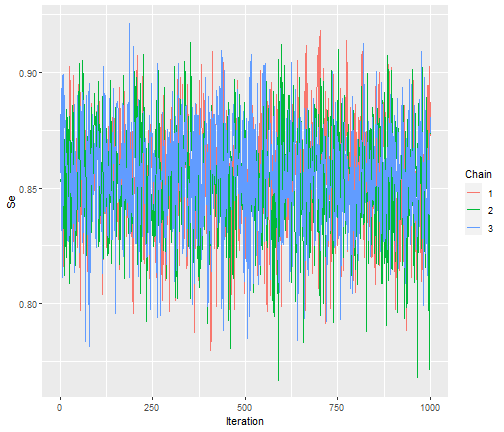
\includegraphics{Session_Preparation_files/figure-latex/unnamed-chunk-23-1.pdf}

The algorithm starts an initial value of prevalence=0.05 at iteration 0.
At each subsequent iteration (x-axis), a new value of prevalence is
chosen based its the posterior probability, although the new value
depends to some extent on the value at the last iteration, which you can
see on the trace plot as autocorrelation (meaning that consecutive
samples are not completely independent). After 1000 iterations, we have
a sample of 1000 values from something that we hope is close to the true
posterior. We can check this by comparing the profiled posterior to a
density plot of the sampled values:

\begin{Shaded}
\begin{Highlighting}[]
\FunctionTok{par}\NormalTok{(}\AttributeTok{mfrow=}\FunctionTok{c}\NormalTok{(}\DecValTok{2}\NormalTok{,}\DecValTok{1}\NormalTok{))}
\FunctionTok{with}\NormalTok{(results, }\FunctionTok{plot}\NormalTok{(parameter, posterior, }\AttributeTok{type=}\StringTok{\textquotesingle{}l\textquotesingle{}}\NormalTok{, }
                   \AttributeTok{xlim=}\FunctionTok{c}\NormalTok{(}\DecValTok{0}\NormalTok{,}\DecValTok{1}\NormalTok{), }\AttributeTok{main=}\StringTok{\textquotesingle{}True posterior\textquotesingle{}}\NormalTok{, }\AttributeTok{ylab=}\ConstantTok{NA}\NormalTok{, }\AttributeTok{xlab=}\ConstantTok{NA}\NormalTok{))}
\FunctionTok{plot}\NormalTok{(}\FunctionTok{density}\NormalTok{(samples), }\AttributeTok{xlim=}\FunctionTok{c}\NormalTok{(}\DecValTok{0}\NormalTok{,}\DecValTok{1}\NormalTok{), }\AttributeTok{main=}\StringTok{\textquotesingle{}Sampled posterior\textquotesingle{}}\NormalTok{, }
     \AttributeTok{ylab=}\ConstantTok{NA}\NormalTok{, }\AttributeTok{xlab=}\ConstantTok{NA}\NormalTok{)}
\end{Highlighting}
\end{Shaded}

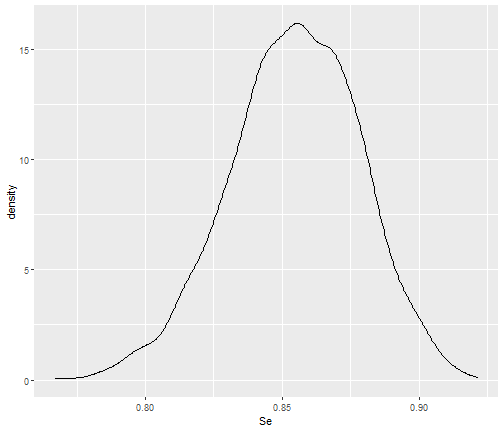
\includegraphics{Session_Preparation_files/figure-latex/unnamed-chunk-24-1.pdf}

They are similar, but not the same. We can also look at estimates of the
mean/median/95\% CI based on the samples

\begin{Shaded}
\begin{Highlighting}[]
\CommentTok{\# Mean of samples:}
\FunctionTok{mean}\NormalTok{(samples)}
\end{Highlighting}
\end{Shaded}

\begin{verbatim}
## [1] 0.6390614
\end{verbatim}

\begin{Shaded}
\begin{Highlighting}[]
\CommentTok{\# Median of samples:}
\FunctionTok{median}\NormalTok{(samples)}
\end{Highlighting}
\end{Shaded}

\begin{verbatim}
## [1] 0.6480227
\end{verbatim}

\begin{Shaded}
\begin{Highlighting}[]
\CommentTok{\# 95\% CI of samples:}
\FunctionTok{HPDinterval}\NormalTok{(samples)}
\end{Highlighting}
\end{Shaded}

\begin{verbatim}
##                lower     upper
## prevalence 0.3489199 0.9048346
## attr(,"Probability")
## [1] 0.95
\end{verbatim}

And compare these to the true values that we calculated earlier using
posterior profiling:

\begin{verbatim}
## True posterior mean: 0.6428571
\end{verbatim}

\begin{verbatim}
## True posterior median: 0.6498366
\end{verbatim}

\begin{verbatim}
## True posterior 95% CI: 0.401307 - 0.8736879
\end{verbatim}

Again, these are close, but not the same. There are two reasons for
this:

1 - We did not remove the burnin period

2 - We do not have a sufficiently high effective sample size

Let's look at how to fix these problems.

\hypertarget{burnin}{%
\subsection{Burnin}\label{burnin}}

When we ran the simulation last time, we set an initial value of 0.05
and it took a little while for the Metropolis algorithm to move away
from this starting value because of the autocorrelation in the chains.
This is OK, but we don't actually want to count this ``burnin'' period
as part of the posterior. So we need to tell the algorithm to run for a
few iterations before starting to sample from the posterior. For
example:

\begin{Shaded}
\begin{Highlighting}[]
\NormalTok{samples }\OtherTok{\textless{}{-}} \FunctionTok{metropolis}\NormalTok{(}\AttributeTok{burnin =} \DecValTok{100}\NormalTok{, }\AttributeTok{sample =} \DecValTok{1000}\NormalTok{, }\AttributeTok{initial\_value=}\FloatTok{0.05}\NormalTok{)}
\end{Highlighting}
\end{Shaded}

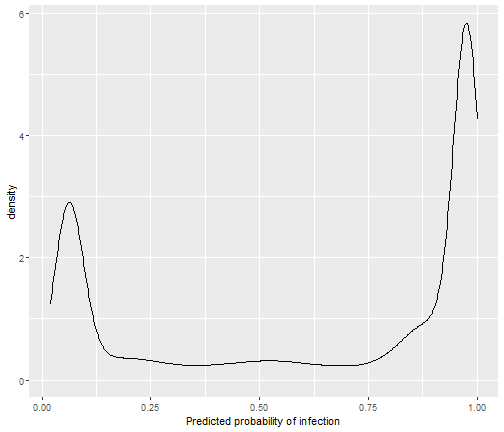
\includegraphics{Session_Preparation_files/figure-latex/unnamed-chunk-28-1.pdf}

This time, we told the function to discard the first 100 samples (shown
in red) and then take another 1000 samples from the posterior after this
point. This means that we can set the initial values to wherever we
want, and it won't affect the samples we take (the blue part) even
though it will affect the burnin period (the red part). For example if
we set an initial value of 0.99:

\begin{Shaded}
\begin{Highlighting}[]
\NormalTok{samples }\OtherTok{\textless{}{-}} \FunctionTok{metropolis}\NormalTok{(}\AttributeTok{burnin =} \DecValTok{100}\NormalTok{, }\AttributeTok{sample =} \DecValTok{1000}\NormalTok{, }\AttributeTok{initial\_value=}\FloatTok{0.99}\NormalTok{)}
\end{Highlighting}
\end{Shaded}

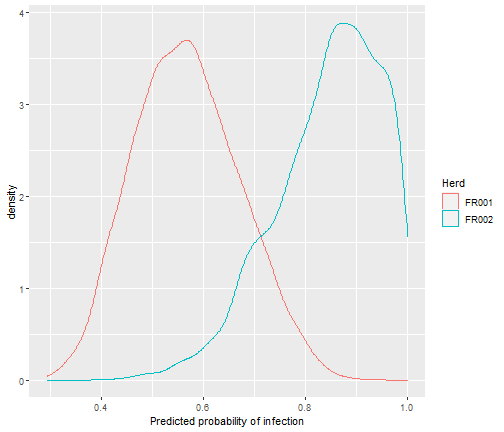
\includegraphics{Session_Preparation_files/figure-latex/unnamed-chunk-30-1.pdf}

The start of the red parts of the chains look quite differnt (one starts
low the other starts high), but by the time it gets to the end of the
red part they seem to be moving around in the same area. At this point
we say that the chains have converged, which is just a fancy way of
saying that it is safe to assume the next samples are from the true
posterior. Note that it doesn't matter if we have a burnin period that
is too long (e.g.~in this case it seems that 50 iterations would have
been enough) - it is far safer to remove more than you think is
necessary rather than risking not removing enough. It is also impossible
to know a priori how long the burnin will take, so if you don't specify
a long enough burnin period then you may have to remove the first part
of the sampled chains manually. This is another reason to err on the
side of caution and specify a longer burnin period than you think will
be needed.

\emph{Important point:} Assessing convergence (and ensuring adequate
burnin) is a crucial (and sometimes tricky) part of using MCMC in
practice.

\hypertarget{effective-sample-size}{%
\subsection{Effective sample size}\label{effective-sample-size}}

Another reason that our samples differed to the true posterior is
because the samples are random, and therefore there is some sampling
noise. In order to eliminate this we need to make sure we have a
sufficient number of samples so that the difference between e.g.~the
mean of the sample and the true mean of the distribution underlying this
sample becomes negligible (or at least small enough for our needs). In
the previous example we had 1000 iterations, but this does not equal
1000 independent samples because of the autocorrelation. Instead we need
to look at the effective sample size:

\begin{Shaded}
\begin{Highlighting}[]
\CommentTok{\# Effective sample size:}
\FunctionTok{effectiveSize}\NormalTok{(samples)}
\end{Highlighting}
\end{Shaded}

\begin{verbatim}
## prevalence 
##   27.06787
\end{verbatim}

So we have the equivalent of approximately 27 independent samples from
this posterior, which is not nearly enough to be a good approximation.
Ideally we would like at least 500 (or even 1000) independent samples,
which means running the simulation for a lot more than 1000 iterations.
For example:

\begin{Shaded}
\begin{Highlighting}[]
\NormalTok{samples }\OtherTok{\textless{}{-}} \FunctionTok{metropolis}\NormalTok{(}\AttributeTok{burnin =} \DecValTok{1000}\NormalTok{, }\AttributeTok{sample =} \DecValTok{20000}\NormalTok{, }\AttributeTok{initial\_value=}\FloatTok{0.05}\NormalTok{)}
\end{Highlighting}
\end{Shaded}

\includegraphics{Session_Preparation_files/figure-latex/unnamed-chunk-33-1.pdf}

\begin{Shaded}
\begin{Highlighting}[]
\CommentTok{\# Effective sample size:}
\FunctionTok{effectiveSize}\NormalTok{(samples)}
\end{Highlighting}
\end{Shaded}

\begin{verbatim}
## prevalence 
##   616.3076
\end{verbatim}

We now have 20000 iterations, which equates to around 616 independent
samples (i.e.~we need around 33 iterations to get 1 independent sample).
This should be enough to get a decent approximation to the true
posterior:

\includegraphics{Session_Preparation_files/figure-latex/unnamed-chunk-34-1.pdf}

\begin{verbatim}
## Mean of samples:  0.6439694
\end{verbatim}

\begin{verbatim}
## True posterior mean: 0.6428571
\end{verbatim}

\begin{verbatim}
## Median of samples:  0.6500875
\end{verbatim}

\begin{verbatim}
## True posterior median: 0.6498366
\end{verbatim}

\begin{verbatim}
## 95% CI of samples:  0.3949136 - 0.8782755
\end{verbatim}

\begin{verbatim}
## True posterior 95% CI: 0.401307 - 0.8736879
\end{verbatim}

Our sampled posterior is now much closer to the true posterior, although
there is still a small difference due to the inherent randomness of the
Monte Carlo integration. This also means that every time we run this
simulation we will get a slightly different answer - if we want to
ensure we get precisely the same result then we need to set the random
number generator seed in R using the set seed function before running
the simulation:

\begin{Shaded}
\begin{Highlighting}[]
\FunctionTok{set.seed}\NormalTok{(}\DecValTok{2021{-}09{-}13}\NormalTok{)}
\NormalTok{samples }\OtherTok{\textless{}{-}} \FunctionTok{metropolis}\NormalTok{(}\AttributeTok{burnin =} \DecValTok{1000}\NormalTok{, }\AttributeTok{sample =} \DecValTok{20000}\NormalTok{,}
                      \AttributeTok{initial\_value=}\FloatTok{0.99}\NormalTok{, }\AttributeTok{plot=}\ConstantTok{FALSE}\NormalTok{)}
\CommentTok{\# Mean of samples:}
\FunctionTok{mean}\NormalTok{(samples)}
\end{Highlighting}
\end{Shaded}

\begin{verbatim}
## [1] 0.6467923
\end{verbatim}

\begin{Shaded}
\begin{Highlighting}[]
\FunctionTok{set.seed}\NormalTok{(}\DecValTok{2021{-}09{-}13}\NormalTok{)}
\NormalTok{samples }\OtherTok{\textless{}{-}} \FunctionTok{metropolis}\NormalTok{(}\AttributeTok{burnin =} \DecValTok{1000}\NormalTok{, }\AttributeTok{sample =} \DecValTok{20000}\NormalTok{,}
                      \AttributeTok{initial\_value=}\FloatTok{0.99}\NormalTok{, }\AttributeTok{plot=}\ConstantTok{FALSE}\NormalTok{)}
\CommentTok{\# Mean of samples:}
\FunctionTok{mean}\NormalTok{(samples)}
\end{Highlighting}
\end{Shaded}

\begin{verbatim}
## [1] 0.6467923
\end{verbatim}

These two results are numerically identical because the same seed was
used. But the following simulation uses a different seed so gives
slightly different results:

\begin{Shaded}
\begin{Highlighting}[]
\FunctionTok{set.seed}\NormalTok{(}\DecValTok{2021{-}09{-}20}\NormalTok{)}
\NormalTok{samples }\OtherTok{\textless{}{-}} \FunctionTok{metropolis}\NormalTok{(}\AttributeTok{burnin =} \DecValTok{1000}\NormalTok{, }\AttributeTok{sample =} \DecValTok{20000}\NormalTok{,}
                      \AttributeTok{initial\_value=}\FloatTok{0.99}\NormalTok{, }\AttributeTok{plot=}\ConstantTok{FALSE}\NormalTok{)}
\CommentTok{\# Mean of samples:}
\FunctionTok{mean}\NormalTok{(samples)}
\end{Highlighting}
\end{Shaded}

\begin{verbatim}
## [1] 0.6521939
\end{verbatim}

\emph{Important point:} MCMC is a numerical approximation to the
posterior, so if we want a good approximation then we need to be sure
our effective sample size is sufficient.

\hypertarget{exercise-1}{%
\subsection{Exercise 1}\label{exercise-1}}

Run the code below with different values of \(sample\). Make sure you
understand the relationship between the number of samples, the effective
sample size, and the accuracy of your estimates from the sampled
posterior:

\begin{Shaded}
\begin{Highlighting}[]
\NormalTok{samples }\OtherTok{\textless{}{-}} \FunctionTok{metropolis}\NormalTok{(}\AttributeTok{burnin =} \DecValTok{1000}\NormalTok{, }\AttributeTok{sample =} \DecValTok{10000}\NormalTok{)}
\CommentTok{\# Effective sample size:}
\FunctionTok{effectiveSize}\NormalTok{(samples)}
\CommentTok{\# Mean of samples:}
\FunctionTok{mean}\NormalTok{(samples)}
\CommentTok{\# Median of samples:}
\FunctionTok{median}\NormalTok{(samples)}
\CommentTok{\# 95\% CI of samples:}
\FunctionTok{HPDinterval}\NormalTok{(samples)}
\end{Highlighting}
\end{Shaded}

Remember the true values for comparison:

\begin{verbatim}
## True posterior mean: 0.6428571
\end{verbatim}

\begin{verbatim}
## True posterior median: 0.6498366
\end{verbatim}

\begin{verbatim}
## True posterior 95% CI: 0.401307 - 0.8736879
\end{verbatim}

\hypertarget{exercise-2}{%
\subsection{Exercise 2}\label{exercise-2}}

Up to now we have not changed the parameter \(sigma\). For the
Metropolis algorithm, the value of \(sigma\) has a big effect on the
degree of autocorrelation in the chains. If the value is either too
large or too small, then there will be a lot of autocorrelation in the
chain, which will result in two things:

1 - The chain might take longer to burn in (particularly if sigma is too
small)

2 - The effective sample size will be reduced

Run the following code with different values of sigma and see how it
affects the autocorrelation. Make sure you understand the relationship
between autocorrelation, the length of the burnin period, and the
effective sample size. Here are some examples to get you started:

\begin{Shaded}
\begin{Highlighting}[]
\CommentTok{\# Large sigma:}
\NormalTok{samples }\OtherTok{\textless{}{-}} \FunctionTok{metropolis}\NormalTok{(}\AttributeTok{sigma=}\DecValTok{10}\NormalTok{)}
\CommentTok{\# Autocorrelation:}
\FunctionTok{autocorr}\NormalTok{(samples, }\AttributeTok{lags=}\DecValTok{1}\NormalTok{)}
\CommentTok{\# Effective sample size:}
\FunctionTok{effectiveSize}\NormalTok{(samples)}

\CommentTok{\# Moderately large sigma:}
\NormalTok{samples }\OtherTok{\textless{}{-}} \FunctionTok{metropolis}\NormalTok{(}\AttributeTok{sigma=}\DecValTok{1}\NormalTok{)}
\CommentTok{\# Autocorrelation:}
\FunctionTok{autocorr}\NormalTok{(samples, }\AttributeTok{lags=}\DecValTok{1}\NormalTok{)}
\CommentTok{\# Effective sample size:}
\FunctionTok{effectiveSize}\NormalTok{(samples)}

\CommentTok{\# Moderately small sigma:}
\NormalTok{samples }\OtherTok{\textless{}{-}} \FunctionTok{metropolis}\NormalTok{(}\AttributeTok{sigma=}\FloatTok{0.1}\NormalTok{)}
\CommentTok{\# Autocorrelation:}
\FunctionTok{autocorr}\NormalTok{(samples, }\AttributeTok{lags=}\DecValTok{1}\NormalTok{)}
\CommentTok{\# Effective sample size:}
\FunctionTok{effectiveSize}\NormalTok{(samples)}

\CommentTok{\# Small sigma:}
\NormalTok{samples }\OtherTok{\textless{}{-}} \FunctionTok{metropolis}\NormalTok{(}\AttributeTok{sigma=}\FloatTok{0.01}\NormalTok{)}
\CommentTok{\# Autocorrelation:}
\FunctionTok{autocorr}\NormalTok{(samples, }\AttributeTok{lags=}\DecValTok{1}\NormalTok{)}
\CommentTok{\# Effective sample size:}
\FunctionTok{effectiveSize}\NormalTok{(samples)}
\end{Highlighting}
\end{Shaded}

Can you find a value of \(sigma\) that gives an effective sample size of
\textgreater= 2000?

\hypertarget{conclusions}{%
\subsection{Conclusions}\label{conclusions}}

In the real world we would very rarely use a Metropolis algorithm, but
it is a useful exercise to understand the basic concepts. You can think
of all other types of MCMC as used by JAGS/BUGS (and also Hamiltonian
Monte Carlo as used by Stan) as being extensions of this same principle.
Crucially, you ALWAYS need to make sure of the following two key points
before trusting any estimates made from your sampled posteriors:

1 - Make sure that the chain(s) have converged, and that a sufficient
burnin period has been run before starting to sample. The two most
common methods of doing this are to look at the potential scale
reduction factor (psrf) of the Gelman-Rubin statistic, and to look at
trace plots (typically of more than 1 independent chain) for each
parameter to make sure the chains have converged on the stationary
posterior. This is extremely important, and can be tricky.

2 - Make sure that you have a sufficient effective sample size. This is
relatively easy to do, simply by remembering to check the effective
sample size (this should be produced by whatever software you are using)
to make sure it is over at least 500 (and preferably 1000) for all
parameters of interest.

We will reinforce these concepts (and show you how to assess them for
models run in JAGS) during the training school.

\end{document}
